\section{Quantum Computing}

Classical computers have been getting exponentially faster over the last 50 years, as observed by Moore's law \cite{Moore1965}. 
Still, it was suggested as early as 1982 that a classical computer may never be efficient at modeling a quantum mechanical system \cite{Feynman1982}. 
This is because of superposition (\cref{sub:Superposition}) and entanglement (\cref{sub:Entanglement}). 
The idea of using a quantum computer is to make use of these very same properties that make a quantum system challenging to simulate, but to use them to one's advantage instead. 
If this would be possible, we can simulate new molecules and chemical reaction mechanisms, opening up the road to novel medicine \cite{Robert2021}, materials \cite{Ma2020} and faster algorithms for machine learning, which would have applications for image recognition, text translation and more \cite{Huang2021}.

\subsection{Superposition}\label{sub:Superposition}

The first reason why quantum computation is fundamentally different from its classical equivalent is superposition.
Consider a single two-level quantum system, quantum bit or \lq qubit' represented by the normalized wave function $\ket{\psi}$, for example, the spin of an electron, which we can define as a basis with basis states $\ket{0}$ (spin-up) and $\ket{1}$ (spin-down). 
According to quantum mechanics, this qubit can be in a superposition state \cite{Griffiths2004}:

\begin{equation}\label{eq:SuperPositionBasic}
	\ket{\psi}=a\ket{0}+b\ket{1},
\end{equation}
where $a,b \in \mathbb{C}$, where one will measure $\ket{0}$ (spin up in this example) with probability $|a|^2$ and and $\ket{1}$ (spin down) with $|b|^2$. 
Without loss of generality, we can let the variable $\theta$ keep track of the probability of measuring $\ket{0}$ or $\ket{1}$, and define $\phi$ as the relative phase between the two, such that the wave function $\psi$ is represented as

\begin{equation}\label{eq:BlochSphere}
	\ket{\psi} = 
	\cos{\frac{\theta}{2}} \ket{0} + e^{i \phi} \sin{\frac{\theta}{2}} \ket{1}.
\end{equation}
This is powerful because we can plot the Hilbert space of the qubit on a unit sphere called the Bloch sphere representation \cite{Nielsen2011}.
This Bloch sphere is shown in \cref{fig:BlochSphere}.
Classical binary bits are shown as well, which in this analogy occupy only the poles of the sphere, whereas the quantum state can be anywhere on this unit sphere. 
This hints at the increased amount of computational information that can be stored in a qubit compared to a classical bit. 

But to build a quantum computer, we are going to need more than one qubit. 
While we cannot easily graphically represent multi-qubit states like for the Bloch sphere, we can still write them down, for which we will introduce the concept of entanglement.

\begin{figure}
	\centering
	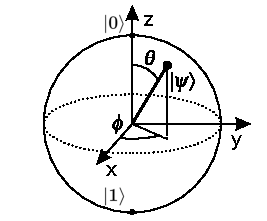
\includegraphics[width=.34\linewidth]{figures/BlochSphereCropped.pdf}
	\caption{The Bloch sphere representation. A classical bit can only be $\ket{0}$ or $\ket{1}$, whereas a qubit can occupy any point on the sphere with coordinates $\theta, \phi$. Figure adapted from \cite{Jones2012}.}
	\label{fig:BlochSphere}
\end{figure}

\subsection{Entanglement}\label{sub:Entanglement}

We will extend from 1 to 2 electrons. 
The electrons are assumed to be distinguishable. 
Now, they can be independently spin up $\ket{0}$ and down: $\ket{1}$, for a total of 4 basis states.
Quantum physics teaches us this system can be in a superposition of all its basis states \cite{Nielsen2011}, which also contains entangled states:

\begin{equation}\label{eq:TwoQubits}
	\ket{\psi_{2q}} = 
	\alpha_{00} \ket{00} + \alpha_{01} \ket{01} + \alpha_{10} \ket{10} + \alpha_{11} \ket{11}.
\end{equation}
Here, $\ket{00}$ is a shorthand notation for both qubits being in the spin-up state, etc.
In general, the size of the Hilbert space will grow as $2^N$ for $N$ qubits \cite{Nielsen2011,Henriet2020}. 
For $N=300$, this is already larger than the estimated amount of particles in the observable universe at some $\sim 10^{80}$. 
Clearly, the number of possible states a realistic atom or molecule can occupy is too large to keep track of for a classical computer.
\Cref{eq:TwoQubits} also contains special states known as entangled states. 
These are an inherent quantum feature, having no classical analog.
One of the most instructive examples of an entangled state is 

\begin{equation}\label{eq:Entangled}
	\ket{\Phi^+} = \frac{1}{\sqrt{2}} \ket{00}+ \frac{1}{\sqrt{2}} \ket{11}.
\end{equation}
This is one of the so-called Bell states \cite{Nielsen2011} and it is said to be entangled: upon measuring just one of the qubits we immediately know the state of the other qubit as well.
This implies the qubits are correlated and cannot be described as a product of independent single qubits.
In the operation of a quantum computer, entanglement is crucial because it allows the quantum register to access the full $2^N$ Hilbert space.
Entanglement is acquired from interactions between neighboring qubits \cite{Henriet2020}.

\section{The NISQ Era}

Apart from controlling the quantum states of individual qubits, qubits are to be shielded from the environment, as noise from the environment can change the quantum states of the qubits. 
This effect is known as decoherence \cite{DiVincenzo2000}. Decoherence errors can be corrected but this requires significant overhead in the available number of qubits and is unachievable in the near term \cite{Peres1985,Ladd2010}. 
Therefore, quantum computing is currently said to be in the \ac{NISQ} \cite{Preskill2018}.
During the NISQ era, the algorithms that run on quantum computers should be optimized for finite coherence times and fidelities. 
One algorithm proposed by \cite{Peruzzo2014} is thought to run especially well on non error-corrected hardware \cite{McClean2016}. We will review the core features of this algorithm here, because it gives insight in the possibilities and limitations of near-term quantum hardware.

\subsection{The Variational Quantum Eigensolver}

The \ac{VQE} is a hybrid quantum algorithm: by making use of classical hardware it aims to reduce the number of quantum gates needed, which is advantageous on NISQ era hardware with finite coherence times \cite{McClean2016}. 
Essentially, VQE tries to find approximately the ground state energy of an atom or molecule according to the variational principle \cite{Griffiths2004}, which states that the expectation value of a given Hamiltonian $\mathcal{H}$ will always be an upper bound for the ground state energy $E_g$:

\begin{equation}\label{eq:VariationalPrinciple}
	\left\langle \mathcal{H} \right\rangle = \bra{\Psi}\mathcal{H} \ket{\Psi} \geq E_g.
\end{equation}
Basically, to solve this problem we need to find the lowest eigenvalue of the (large) matrix $\mathcal{H}$. 
Even for relatively simple molecules, $\mathcal{H}$ quickly becomes large and the task of diagonalizing it intractable, at least for a classical computer.
In \ac{VQE}, $\mathcal{H}$ is not directly diagonalized but the Hamiltonian is prepared in a quantum co-processor or \ac{QPU} \cite{Henriet2020,Peruzzo2014}, taking advantage of the large Hilbert space of the quantum hardware.
Given an ansatz $\theta$, a trial state $\ket{\Psi(\theta)}$ is prepared.
The Hamiltonian is written in the form of a sum of Pauli strings: $P_{\alpha}$ with weights $h_{\alpha}$ \cite{McClean2016,Moll2018}

\begin{equation}
	\mathcal{H} = \sum_{\alpha} h_{\alpha} P_{\alpha}.
\end{equation}
A Pauli string is a tensor product of Pauli spin matrices $\sigma_j^{\alpha} \in \{\mathcal{I}, \sigma_j^x, \sigma_j^y, \sigma_j^z\}$ \cite{Griffiths2004}:

\begin{equation}\label{eq:PauliString}
	P_{\alpha} = 
	\sigma_1^{\alpha_1} \otimes \sigma_2^{\alpha_2} \otimes \ldots \otimes \sigma_N^{\alpha_N} = 
	\bigotimes_{j=1}^N \sigma_j^{\alpha_j}.
\end{equation}
We will not delve further in theoretical details. 
But what it boils down to is that because of this decomposition, estimating the various terms of the Hamiltonian $\bra{\Psi} P_{\alpha} \ket{\Psi}$ corresponds to measuring populations of individual qubits.
The total expectation value of the Hamiltonian is obtained by summing over contributions of the Pauli strings.
This is done on classical hardware.
Subsequently, a non-linear optimizer is run to minimize the energy using a new trial state, which is fed back into the \ac{QPU}.
\cite{Moll2018}. 
The quantum and classical components of the algorithms feed into each other, therefore \ac{VQE} is referred to as a hybrid algorithm. 
The algorithm is visualized in \cref{fig:VQE}.

\begin{figure}
	\centering
	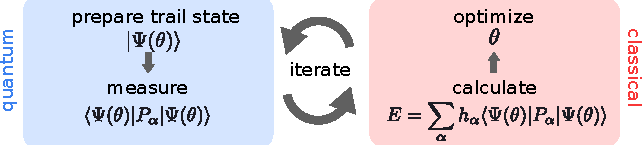
\includegraphics[width=0.89\linewidth]{figures/VQE.pdf}
	\caption{The \ac{VQE} visualized. 
	Meant to run on a hybrid quantum computer, starting from an ansatz for the wave function it is prepared and the expectation function of its energy measured by a series of measurements on the \ac{QPU}.
	Next, a CPU uses a non-linear optimization to find a new ansatz that will decrease the expectation value of $\mathcal{H}$. Iterated until convergence. Figure adapted from \cite{Moll2018}.}
	\label{fig:VQE}
\end{figure}

\section{Hardware Implementation}

There are many options for implementing the algorithm on quantum hardware.
A list of requirements the hardware should adhere to were formulated by \cite{DiVincenzo2000} .
Based on this, several quantum computer realizations have been proposed \cite{Ladd2010}.
Examples include infrared photons \cite{Matthews2009}, trapped ions \cite{Benhelm2008,Schindler2013}, electron spins \cite{Press2008} and superconducting currents \cite{DiCarlo2009,Arute2019}. 
This work is about another platform: using ultracold atoms as qubits. 

\subsection{Ultracold Atoms}

When using ultracold atoms, the qubit states are encoded in electronic states of neutral atoms, which are cooled to temperatures just above the absolute zero to minimize decoherence effects. 
These atoms are assembled in arbitrary geometries using laser cooling and trapping techniques.
One of those techniques is using tightly focused laser beams to trap atoms, also known as optical tweezers.
Each optical tweezer or optical dipole trap \cite{Chu1986} is loaded non-deterministically with single atoms \cite{Schlosser2001}. 
Multiple dipole traps spaced a couple of micrometers from each other are generated using holography techniques \cite{Bergamini2004}.
Interactions between qubits are realized using excitation to very high principle quantum numbers (Rydberg states) \cite{Levine2018,Madjarov2020}. 
Lastly, projections of qubit states are measured using laser induced fluorescence.
An overview of the different steps in neutral atom quantum computing is shown in \cref{fig:ComputingSteps}.

One of the advantages of this platform is that is is rather flexible: the amount of qubits, lifetimes, coherence times and degree of interaction can be tuned by changing parameters of the lasers used. 
Additionally, neutral atoms are shielded quite well from the environment.
Lastly, the technique is thought to easily scale to a higher number of qubits by increasing the trapping laser power \cite{Henriet2020}.

\begin{figure}
	\centering
	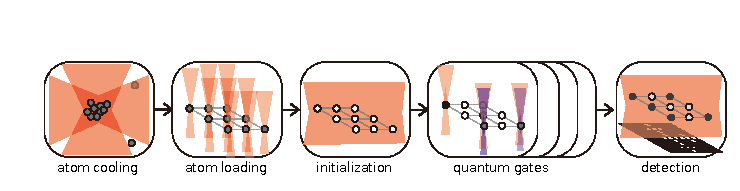
\includegraphics[width=\linewidth]{figures/ComputingSteps.pdf}
	\caption{Steps involved in running a \ac{QPU} based on neutral atoms in optical tweezers. 
	This work concerns the first steps: cooling to ultracold temperatures and loading in an array of optical tweezers.
	Figure from \cite{Wu2021}.}
	\label{fig:ComputingSteps}
\end{figure}

\section{This Thesis}

In a collaboration with the \textit{Schreck} group at the University of Amsterdam, we aim to realize a \ac{QPU} based on neutral atoms, which was recently shown to achieve high-fidelity quantum gates and measurements \cite{Madjarov2020}. 
The purpose of this thesis is to give an update of the first steps carried out in our group towards this goal.
Therefore, this work is mostly about the first two steps in \cref{fig:ComputingSteps}: specifically on how to cool the atoms to ultracold temperatures and how to load them in an array of optical traps known as optical tweezers.
As an atom source, we initially used \ac{Rb}, but plan to move to \ac{Sr} because the energy level structure of Sr is suitable to use as a qubit. 
To to this the work is organized in the following way:

\begin{itemize}
	\setlength\itemsep{-1pt}
	\item Background information about laser cooling and trapping techniques, as well as for Rb and Sr specifically is presented in \cref{ch:coolingtrapping}. 

	\item Chapter \ref{ch:tweezer} is about focusing a laser beam to the smallest possible spot inside of a vacuum chamber, to realize an optical tweezer.

	\item Next, chapter \ref{ch:arrays} elaborates on how to make arrays of tweezers in arbitrary geometries by using holography techniques.

	\item Finally, in \cref{ch:implementation} we describe how the optics used in the previous chapters is implemented in a cold atom experiment. 
	The atom source used for this is Rb, but the platform should work with Sr as well. 
\end{itemize}










